\section{Expériences empiriques}

Cette section sera l'occasion de valider numériquement les garanties présentées à la \cit
quant aux erreurs de généralisation et de sous optimalité inhérentes à l'algorithme
d'investissement présenté dans ce mémoire.

Il va sans dire que le cadre théorique général qui a été développé jusqu'à maintenant
présente plusieurs paramètres (dimensionalité du problème, loi de marché, fonction
d'utilité, noyau employé, etc.); tous les décrire représenterait une tâche titanesque,
aussi certains choix devront être faits pour restreindre la quantité de paramètres
étudiés; la Section \ref{emp:metho} énumérera le choix fait pour chacun de ces paramètres.

Par la suite, les Sections \ref{emp:nvar}, \ref{emp:pvar} et \ref{emp:npvar} étudieront la
qualité des garanties de généralisation et de sous optimalité dans un contexte où,
respectivement, la taille de l'échantillonage augmente, la taille de l'échantillonage est
fixe mais la dimensionalité du problème augmente et enfin, la taille de l'échantillonage
et de la dimensionalité augmentent toutes les deux, mais à des rythmes différents. 


\subsection{Méthodologie}
\label{emp:metho}

\paragraph{Noyau}

Le noyau employé dans nos expériences sera linéaire. En particulier, c'est avec un tel
noyau que la dépendance entre la dimensionalité du problème est les erreurs de sous
optimalité et de généralisation est la plus facilement caractérisable.

\paragraph{Fonctions d'utilité}

Chaque expérience sera conditionnée par une fonction d'utilité exponentielle Lipschitz
$\LEU_\mu$ (voir \figref{fig_leus} pour une description de cette famille).

Ces utilités sont idéales pour deux raisons: d'abord elles ont toutes un coefficient
Lipschitz $\gamma = 1$; ensuite, leur paramètre $\mu\geq0$ permet de quantifier facilement
l'aversion au risque qu'elles convoient, $\mu \to \infty$ correspondant à une attitude neutre au
risque et $\mu = 0$ correspondant à l'attitude extrêmement averse où aucune utilité n'est
accordée aux rendements supérieurs à zéro. Mathématiquement, les fonctions exponentielles
Lipschitz sont définies par
\begin{equation}
  \LEU_\mu(r) = 
  \begin{cases}
    r & r<0\\
    \mu(1-e^{-r/\mu}) & r\geq 0
  \end{cases}.
\end{equation}

La fonction d'utilité inverse $\LEU_\mu^{-1}:\Ut\to\R$, nécessaire pour exprimer en terme de
rendement équivalent les erreurs exprimées en util, est illustrée à la
\figref{fig_leu_inv}. On peut vérifier algébriquement que
\begin{equation}
  \LEU_\mu^{-1}(r) =
  \begin{cases}
    r & r<0\\
    -\mu\log(1-r/\mu) & r\geq 0
  \end{cases}.
\end{equation}

Finalement, les bornes d'erreur de généralisation et de sous optimalité, lorsqu'elles sont
exprimées en équivalent certain, font intervenir l'inverse du sous-gradient de
$u^{-1}$. Dans le cas de l'utilité LEU, celui-ci correspond tout simplement à l'inverse de
la dérivée de $\LEU_\mu$ et est donc donné par
\begin{equation}
  \left(\frac{d}{dr} LEU^{-1}_\mu(r)\right)^{-1} = 
  \begin{cases}
    1 & r<0\\
    e^{r/\mu} & r\geq 0
  \end{cases}.
\end{equation}


\paragraph{Régularisation}

Sauf exception, le facteur de régularsation $\lambda = 1/2$ sera employé au cours de toutes les
expériences. 



\paragraph{Loi de marché}

La loi de marché $M$ sera construite en deux temps. D'abord, une loi de marché théorique
$\tilde M \in \Re^{p+1 \times p+1}$ sera définie. Toutes ses marges seront décrites par des
variables aléatoires Rademacher (retournant $\pm 1$ avec probabilité $1/2$). La dépendance
entre les marges sera modélisée à l'aide d'une copule gaussienne dont la matrice de
corrélation sera définie en début de chaque section.

Puis, à partir de cette loi de marché théorique $\tilde M$, un échantillon fini
$M \sim \tilde M^{\num{5000}}$ de \num{5000} points en sera tiré afin de former une loi de
marché discrète $M$ à partir de laquelle toutes les expériences seront réalisées. En
quelque sorte, $M$ fournira alors une approximation à $\tilde M$, mais permettra de
déterminer exactement des variables comme l'utilité hors échantillon $\EU(q)$ d'une
politique $q$ ou l'utilité espérée optimale $\nEU^\star$, qu'il serait autrement impossible à
déterminer théoriquement (sauf dans le cas de l'utilité neutre au risque).


\paragraph{Précision de la borne et quantiles d'erreur}

Les bornes sur les erreurs présentées aux Théorèmes \cit s'appliquent à tout échantillon
$\S_n$ avec une probabilité $1-\delta$. Elles s'appliquent donc, de façon équivalente, au
$1-\delta$-ième quantile avec probabilité 1.

Ainsi, pour confirmer ces bornes, celles-ci seront évaluées à $\delta = 5\%$ et le 95\ieme
percentile d'erreur sera mesuré.

\paragraph{Échantillonnage}

Les échantillons d'entraînement $\S_n$ seront traités de façon équivalente pour toutes les
sections.

Par exemple, à la Section \ref{emp:nvar}, où c'est la taille de l'échantillon qui augmente
linéairement, on tirera d'abord $m \times \bar n$ réalisations de $M$ afin d'obtenir $m$
échantillons d'entraînement $\S_{\bar n}$. Puis, on exposera progressivement à
l'algorithme $n$ des $\bar n$ points afin d'obtenir peu à peu une meilleure représentation
de $M$. Les $m$ points serviront à déterminer le 95\ieme percentile d'erreur.

À la Section \ref{emp:pvar}, où c'est la dimensionalité du problème qui varie, l'idée
demeure la même, cette fois avec $n$ fixe et $p$ variable. On tire donc tout d'abord
$m\times\bar n$ réalisations de $M$. Comme chacune de ces réalisations est consituée de $\bar
p$ variables d'information, où $\bar p$ note le nombre de marges d'information de $M$, on
a alors qu'à présenter à l'algorithme des réalisations ``incomplètes'', dont seules les
$p$ premières dimensions sont connues.

Enfin, à la section \ref{emp:npvar}, la situation est un mélange des deux précédentes, où
de plus en plus de points provenant d'un même échantillon sont présentés à l'algorithme,
leur dimension dévoilée progressant en fonction de $n$. 

Toutes nos expériences disposeront de $m=100$ échantillons d'entraînement.



\paragraph{Environnement de calcul}

L'identification numériques des politiques optimales $\qh$ se fera à partir de
l'implémentation CVXPY\cite{cvxpy} et du solveur ECOS\cite{ecos}. Les calculs numériques
se feront à partir de la librairie BLAS et de l'interface NUMPY.

\newpage

\begin{figure}[ht]
  \centering
  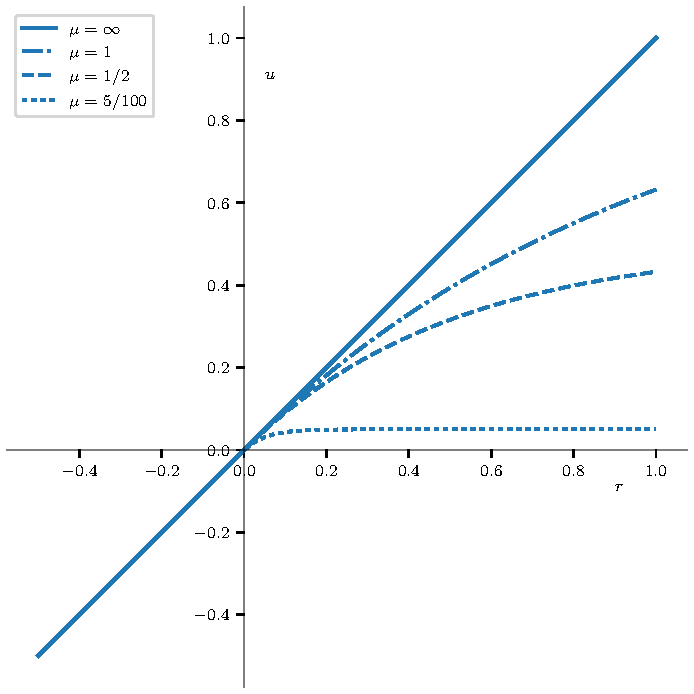
\includegraphics[width=\textwidth]{../../experiments/fig/leus.pdf}
  \caption[Utilités LEU]{Fonctions d'utilité exponentielles Lipschitz (LEU)}
  \label{fig_leus}


  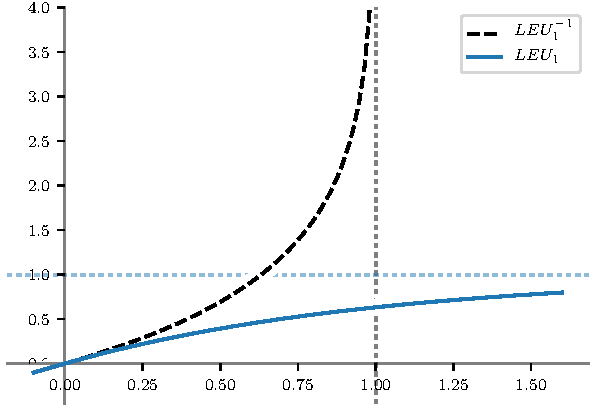
\includegraphics[width=\textwidth]{../../experiments/fig/leu_inv.pdf}
  \caption{Utilité et utilité inverse}
  \label{fig_leu_inv}
\end{figure}

\clearpage


\subsection{\textit{n} variable, \textit{p} constant}
\label{emp:nvar}

L'objet de cette section est l'étude du cas canonique où la taille $n$ de l'échantillon
$\mathcal{S}_n$ augmente linéairement.

\paragraph{Loi de marché}

Tel qu'expliqué à la Section \ref{emp:metho}, une loi de marché discrète $M$ sera dérivée
d'une loi théorique $M$. Cette loi théorique disposera ici de trois marges (deux variables
d'information et une variable de rendement, toutes trois Rademacher). La loi théorique de
marché $M$ sera modélisé à partir de la matrice corrélation $\Sigma$ donnée par
\begin{equation}
  \Sigma  =
  \kbordermatrix{
    & X_1 & X_2 & R\\
    X_1 & 1 & 0 & \rho\\
    X_2 & 0 & 1 & \rho\\
    R & \rho & \rho &1},
\end{equation}
où $\rho = 1/\sqrt{2}$, ce qui correspond à la plus grande valeur de corrélation permettant à
$\Sigma$ d'être semi-définie positive.  Ainsi, $X_1$ et $X_2$ seront mutuellement indépendants,
mais auront toutes deux une influence égale sur la réalisation de $R$ (la corrélation
entre $X_j$ et $R$ correspond au tau de Kendall: $\Corr(X_j,R) =
\frac{2}{\pi}\arcsin(\rho) = 1/2$. Voir \cite{remillard2013statistical} pour des précisions).

On en déduit évidemment que $\xi = \sqrt{2}$ et $\rmax = 1$. 


\subsubsection{Erreur de généralisation}

On rappelle que l'erreur de généralisation d'une politique d'investissement $q$ consiste à
mesurer la différence entre l'utilité (resp. équivalent certain) espérée observée en
échantillon avec l'utilité (resp. équivalent certain) espérée hors échantillon, ou,
mathématiquement, de déterminer $\hEU(q) - \EU(q)$ (resp. $\hCE(q) - \CE(q)$).

\paragraph{Quantiles d'erreur -- Figure \ref{fig_genstats}}

Tout d'abord, la \figref{fig_genstats} indique les quantiles d'erreur de généralisation
des $m$ échantillons d'entraînement, incluant la valeur maximale et minimale pour chaque
$n$. Nos bornes ne donnent que des garanties partielles sur les maximums ni sur les
minimums, cependant il est intéressant d'observer le comportement convergenant vers zéro
de chacun des quantiles d'erreur. 

\paragraph{Erreur de généralisation et aversion au risque -- Figure \ref{fig_avrisk_gen}}

Par ailleurs, si intuitivement on peut s'attendre à observer une relation entre l'erreur
de généralisation et l'aversion au risque, la \figref{fig_avrisk_gen} montre
qu'effectivement, une plus forte aversion au risque (caractérisée par $\mu$) entraîne une
erreur de généralisation plus faible, alors qu'au contraire, une faible aversion au risque
entraîne une erreur de généralisation plus importante. Cette relation est importante
puisqu'elle permet de généraliser les observations empiriques faites à partir d'une seule
utilité à d'autres utilités. Dans les expériences suivantes, l'utilité étalon sera celle
caractérisée par un coefficient $\mu=1$.

\paragraph{Borne sur l'erreur -- Figures \ref{fig_bound_errgen} et \ref{fig_bound_gencomps}}

La \figref{fig_bound_errgen} permet de constater la validité des garanties théoriques
offertes par l'algorithme d'investissement. On constate ici que la borne n'est pas
exactement serrée, les courbes théoriques et empiriques différant d'un ordre de
grandeur. Néanmoins, il faut conserver à l'idée que ces bornes sont valides pour toute
distribution de marché $M$ de dimension $\xi\leq\sqrt{2}$ et $\rmax\leq 1$ et toute courbe
d'utilité $u$ de coefficient Lipschitz 1. C'est toutefois avec cette forme particulière de
$M$ (marges Rademacher) qu'on a pu observer les bornes plus serrées. 

Ceci dit, si les bornes ne sont en tant que telles pas particulièrement fortes, l'ordre
$\bigO(n^{-1/2})$ qu'elles indiquent est lui très bien respecté empiriquement et il pourrait
donc être possible d'anticiper de combien l'erreur empirique peut décroître selon la
taille de l'échantillonnage en interpolant tout simplement les erreurs déjà
observées avec un polynôme $\bigO(n^{-1/2})$. 

\paragraph{Erreur en util et en équivalent certain}

Quant à l'erreur théorique et sa borne, on constate qu'il y a en fait peu de distorsion
entre le domaine de l'util et celui du rendement. Pour expliquer ce phénomène, la
\figref{fig_bound_gencomps} décompose l'erreur de généralisation : d'une part sa partie
erreur en échantillon et hors échantillon. On y observe que les valeurs obtenues en util,
toutes inférieures à \num{0.6}, entraînent une faible distorsion si on se fie à la
\figref{fig_leu_inv}.


\newpage


\begin{figure}[h!]
  \centering
  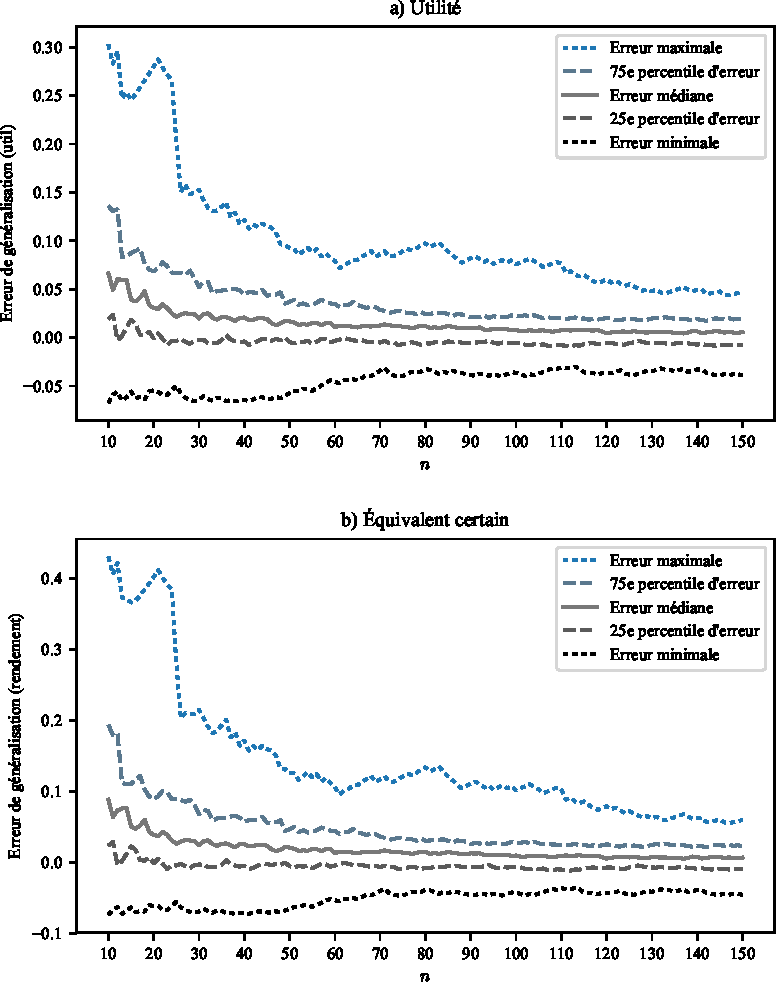
\includegraphics[width=\textwidth]{../../experiments/fig/genstats.pdf}
  \caption{Quartiles et valeurs maximales de l'erreur de généralisation}
  \label{fig_genstats}
\end{figure}


\begin{figure}[h!]
  \centering
  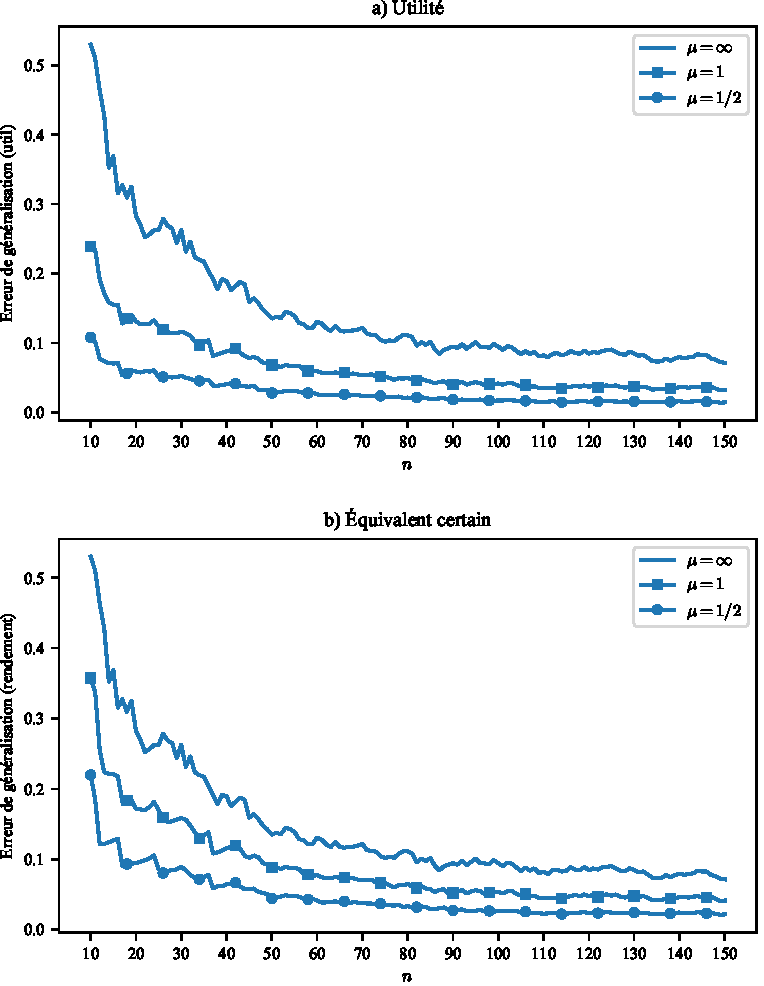
\includegraphics[width=\textwidth]{../../experiments/fig/avrisk_gen.pdf}
  \caption[Aversion au risque et erreur de généralisation]{Aversion au risque et erreur de
    généralisation (95\ieme percentile)}
  \label{fig_avrisk_gen}
\end{figure}



\begin{figure}[h!]
  \centering
  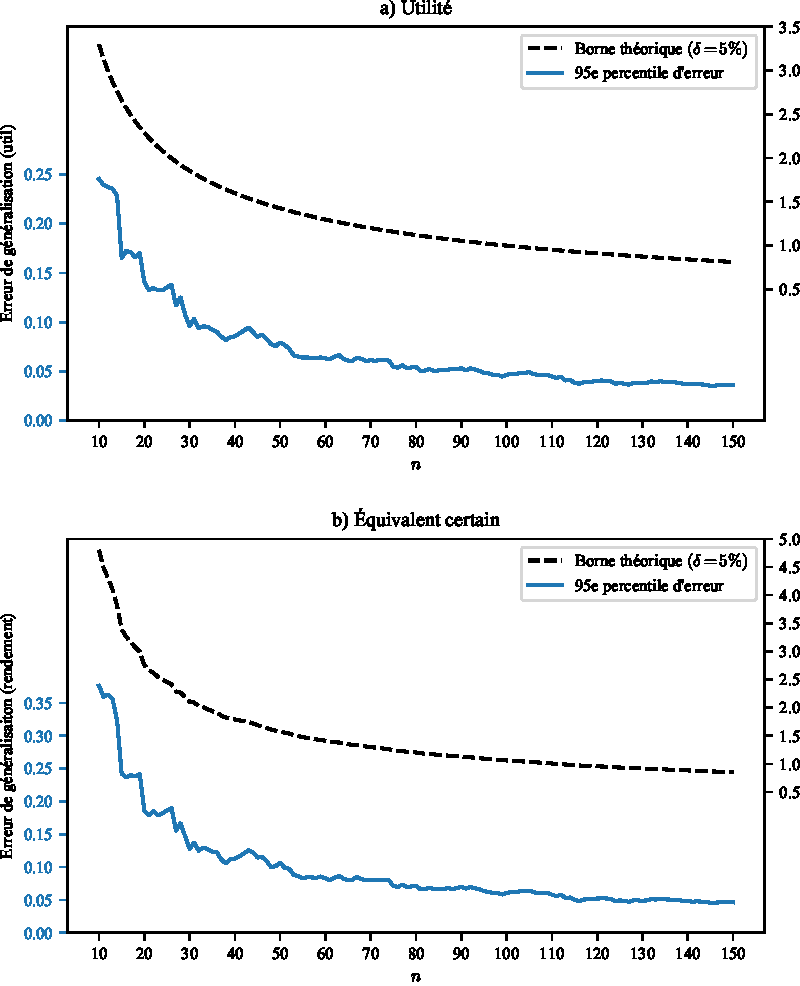
\includegraphics[width=\textwidth]{../../experiments/fig/bound_errgen.pdf}
  \caption[Borne théorique sur l'erreur de généralisation]{Borne sur le 95\ieme percentile
    de l'erreur de généralisation. L'axe de gauche indique la valeur de l'erreur
    empirique, tandis que l'axe de droite indique celle de la borne théorique.}
  \label{fig_bound_errgen}
\end{figure}

\begin{figure}[h!]
  \centering
  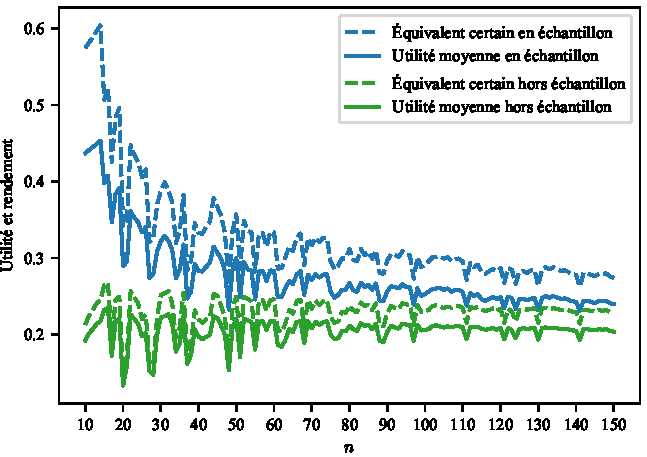
\includegraphics[width=\textwidth]{../../experiments/fig/bound_gencomps.pdf}
  \caption[Composantes de l'erreur maximale]{Composantes en échantillon et hors
    échantillon de l'erreur maximale.}
  \label{fig_bound_gencomps}
\end{figure}

\clearpage


\subsubsection{Erreur de sous optimalité}

\paragraph{λ constant -- Figure \ref{fig_bound_errso}}

Contrairement à l'erreur de généralisation, l'erreur (en util) de sous optimalité
$\EU(\qs) - \EU(\qh)$ (resp.~$\CE(\qs) - \CE(\qh)$ dans le domaine des rendements) ne
bénéficie pas d'une convergence vers zéro du fait de la présence du terme de
régularisation dans l'algorithme $\alg(\S_n)$. En fait, tel que vu au théorème \cit, pour
$n\to\infty$, la meilleure borne qu'on puisse avoir est proportionelle à
$\lambda\|\qs\|^2$ (domaine des utils).

Par exemple la \figref{fig_bound_errso} illustre précisément comment les erreurs
empiriques et théoriques plafonnent toutes les deux à des constantes non nulles. De plus,
contrairement à la borne de généralisation, la borne de sous-optimalité se trouve à deux
ordres de grandeur de l'erreur empirique. Ceci a un effet particulièrement néfaste
lorsqu'on considère la borne dans le domaine des rendements où l'effet de l'utilité
inverse (voir \figref{fig_leu_inv}) se fait violemment sentir: puisque l'utilité de la
politique optimale est proche de la limite asymptotique
$\lim_{r\to\infty}\text{LEU}_1(r) = 1$, l'inversion $u^{-1}(EU^\star)$ retourne une valeur très
élevée.

Néanmoins, tout comme c'était le cas pour l'erreur de généralisation, si la borne de sous
optimalité ne donne pas nécessairement de fortes garanties, en revanche elle suggère un
ordre de convergence qui lui semble être en adéquation avec l'erreur de sous optimalité
empirique maximale (ou plutôt, avec son 95\ieme percentile d'erreur).


\paragraph{λ décroissant -- Figure \ref{fig_bound_errso_lambda}}

Comme il fut discuté à la section \cit, en utilisant un facteur de régularisation
$\lambda = \bigO(n^{-1/2})$, on peut garantir une convergence de l'erreur de sous optimalité
vers zéro (voir \figref{fig_bound_errso_lambda}). Cependant, si dans ce cas-ci l'erreur
empirique de sous-optimalité, qu'elle soit exprimée en util ou en rendement, semble bien
converger à un rythme $\bigO(n^{-1/2})$, la borne théorique elle ne progresse qu'à un
rythme de $\bigO(n^{-1/4})$, ce qui est particulièrement lent. Par contre, même une
progression aussi lente permet quand même d'obtenir des garanties d'équivalent certain un
peu plus raisonnables puisqu'on force alors la limite $\lambda\|\qs\|^2$ de la borne en util à
s'éloigner de la région où $u^{-1}$ retourne des valeurs très grandes.

Par contre, si cette décroissance de $\lambda$ entraîne une convergence de l'erreur de sous
optimalité, c'est au prix de la garantie sur l'erreur de généralisation, qui est elle
proportionelle à $\bigO(\lambda^{-1})$.


\newpage

\begin{figure}[h!]
  \centering
  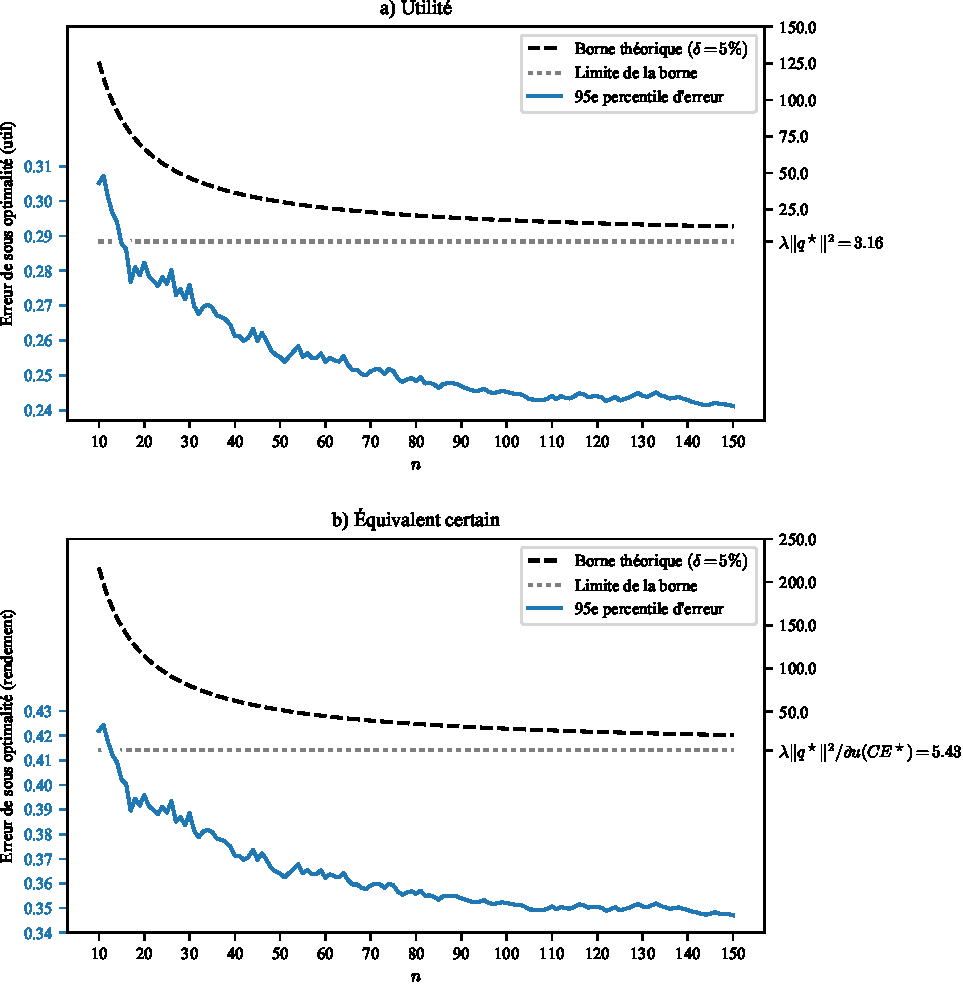
\includegraphics[width=1\textwidth]{../../experiments/fig/bound_errso.pdf}
  \caption{Borne de sous optimalité, $\lambda$ constant}
  \label{fig_bound_errso}
\end{figure}

\begin{figure}[h!]
  \centering
  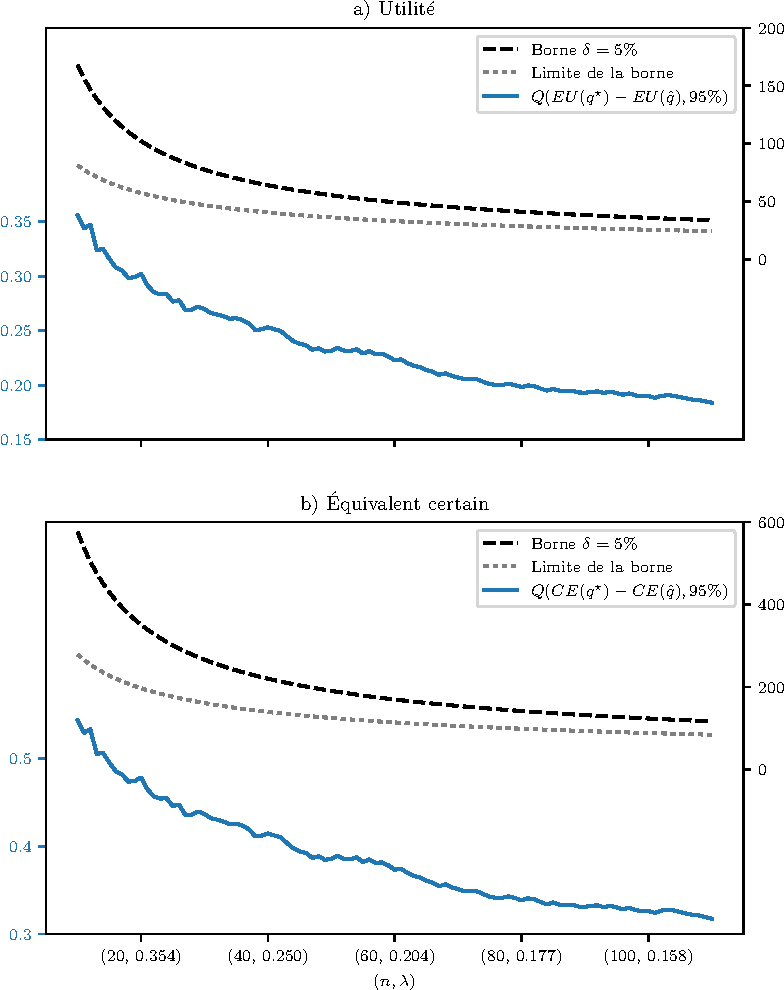
\includegraphics[width=1\textwidth]{../../experiments/fig/bound_errso_lambda.pdf}
  \caption{Borne de sous optimalité, $\lambda$ décroissant}
  \label{fig_bound_errso_lambda}
\end{figure}


\clearpage

\subsection{\textit{n} constant, \textit{p} variable}
\label{emp:pvar}

On peut aussi considérer le rapport qu'entretiennent les bornes de généralisation et de
sous-optimalité de l'algorithme de maximisation d'utilité régularisé lorsqu'on ajoute de
nouvelles informations indépendantes des précédantes, tout en conservant la taille
d'échantillonnage constante.

\paragraph{Protocole d'expérience}

Afin de bien comprendre l'effet que peut avoir un régime en haute dimension sur les deux
types d'erreur étudiées, une copule gaussienne avec marges Rademacher sera encore employée
pour modéliser $\tilde M$. Cette fois cependant, cette copule disposera de $\bar p$ marges
d'information indépendantes dont chaque marge sera dévoilée progressivement. De plus,
trois situations seront étudiées : celle où toute l'information est concentrée à la
première marge, les autres étant indépendantes de $R$, celle où chaque marge dispose d'une
corrélation de $1/\sqrt{\bar p}$ avec $R$ (information dispersée) et finalement celle où
aucune information n'est présente pour déterminer $R$, c'est-à-dire que toutes les marges
$X_j$ sont indépendantes de $R$.

Mathématiquement, $\tilde M$ est donc décrit par une copule gaussienne à $\bar p+1$ marges
Rademacher dont la matrice de corrélation est paramétrée par un vecteur de corrélation $\rho
\in \Re^{\bar p}$:
\begin{equation}
  \Sigma =
  \kbordermatrix{
    &X_1 & \cdots & X_{\bar p} & R\\
    X_1& \ddots & & & \rotatebox{90}{\text{---}}\\
    \vdots  & & I_{\bar p\times \bar p} && \rho\\
    X_{\bar p}&&&\ddots &\rotatebox{90}{\text{---}}\\
    R & \text{---} & \rho & \text{---} &1}.
\end{equation}
Le cas de l'information concentrée se traduira par un vecteur de corrélation donné par
\begin{equation}
  \rho =
  \begin{pmatrix}
    1 & 0 &\cdots &0
  \end{pmatrix},
\end{equation}
celui de l'information dispersée par le vecteur de corrélation
\begin{equation}
  \rho =
  \begin{pmatrix}
    1/\sqrt{\bar p} & \cdots & 1/\sqrt{\bar p}
  \end{pmatrix},
\end{equation}
et celui sans aucune information par le vecteur de corrélation
\begin{equation}
  \rho =
  \begin{pmatrix}
    0 &\cdots &0
  \end{pmatrix}.
\end{equation}
Enfin, les expériences qui suivent fixent le nombre total de variables d'information à
$\bar p =50$.


\paragraph{Erreur de généralisation -- Figure \ref{fig_pconst_infogen}}

On a déjà remarqué que la borne de généralisation affiche une croissance $\bigO(\xi^2)$
ce qui, dans le cas d'un noyau linéaire, devrait se traduire par une progression linéaire
$\bigO(p)$. Ainsi, la \figref{fig_pconst_infogen} montre effectivement une telle
progression pour les trois situations énumérées à la section précédante. 

En fait, la plupart des observations qui ont été faites dans le cas où $p$ est constant et
$n$ est variable peuvent être réutilisées. Par exemple, on remarque que la même différence
d'un ordre de grandeur entre l'erreur empirique et théorique persiste à mesure qu'on
dévoile de nouvelles variables d'informations $X_j$. Et ici encore, on perçoit une faible
dilatation de valeur entre la borne exprimée en util et en rendement.

Pour ce qui concerne les trois situations d'information, bien que chacune d'entre elles
affichent à peu près la même progression linéaire, la situation où toute l'information est
concentrée dès $p=1$ entraîne d'abord une erreur nulle, qui augmente à mesure que de
nouvelles variables ``de bruit'' sont ajoutées. On remarquera par ailleurs la forte
similarité entre les courbes \textit{Information dispersée} et \textit{Aucune
  information}. En effet, comme $\bar p$ est assez important, lorsque $p=1$ et que le
signal est dispersé, le signal perçu à partir d'une seule caractéristique est très
faible. Néanmoins, la courbe d'information diluée fléchit par rapport à celle de l'absence
complète d'information à mesure que $p$ augmente vers $\bar p$, conformément à l'intuition
qu'on pourrait en avoir.

\newpage

\begin{figure}[h!]
  \centering
  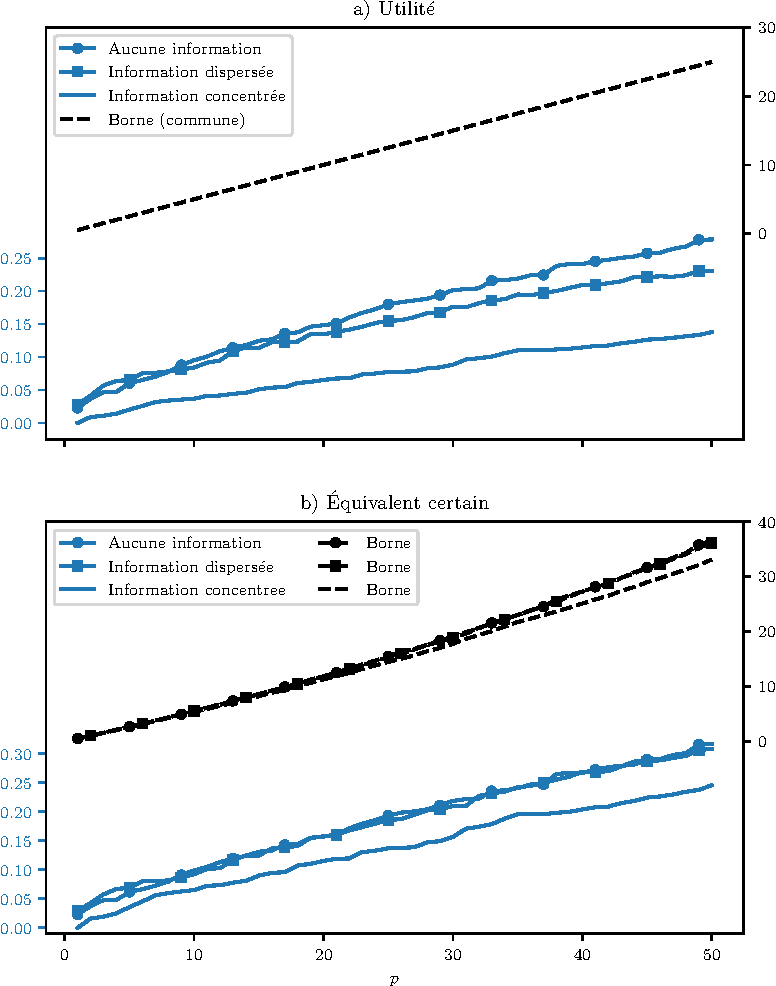
\includegraphics[width=1\textwidth]{../../experiments/fig/pconst_infogen.pdf}
  \caption{Erreur de généralisation avec ajout d'information}
  \label{fig_pconst_infogen}
\end{figure}

\clearpage

\subsubsection{Sous optimalité}

\paragraph{Utilité espérée optimale}

Dans le cas où on ajoute de l'information, la sous optimalité, contrairement à l'erreur de
généralisation, peut référer à deux types d'erreur. Soit on compare la performance hors
échantillon de $\qh$ à celle de la politique optimale qui ne dispose que de $p < \bar p$
variables d'information, soit à la politique optimale qui dispose de $\bar p$ variables
d'information nécessaires pour décrire $M$. Cependant, le développement théorique qui a
été mené au cours de la dernière section ne s'est implicitement préoccupé que de la
première situation.

Par exemple, la \figref{fig_pconst_euinforelative} indique la progression de l'utilité
espérée optimale à mesure que de nouvelles variables d'information sont dévoilées. On y
observe sans surprise que le cas où toute l'information est disponible dès $p=1$ affiche
une utilité espérée optimale constante, alors qu'on a une progression à peu près linéaire
lorsqu'on dévoile progressivement des variables d'information qui sont chacunes faiblement
corrélées à $R$, mais indépendantes l'une à l'autre. Enfin, aucune information se traduit
inévitablement par une utilité espérée optimale nulle.

\paragraph{Erreurs de sous optimalité}

La \figref{fig_pconst_infosorelative} elle, indique la sous optimalité relative à mesure
que de nouvelles variables d'information sont dévoilées. On y note d'abord une progression
de l'erreur pour les trois situations étudiées; de plus, la différence entre le panneau a)
de la Fig.~\ref{fig_pconst_infosorelative} et la Fig.~\ref{fig_pconst_euinforelative} est
une manifestation de la présence du facteur de régularisation constant à mesure que $p$
augmente. Finalement, si les courbes \textit{information dispersée} et \textit{aucune
  information} subissent peu de distortion entre le domaine des utils et celui des
rendements, la courbe \textit{information concentrée} affiche une énorme sous optimalité
lorsqu'elle est exprimée en rendement. Cela s'explique par le fait que $\nEU^\star$ est très
proche de $1$ (numériquement $1-\nEU^\star = \num{1.89e-10}$ lorsque $p=50$), ce qui entraîne
un équivalent certain de l'ordre de \num{10}, puisque $\nCE^\star = -\log_e(\num{1.89e-10})$.


\paragraph{Borne sur l'erreur de sous optimalité -- Figures \ref{fig_pconst_so_conc},
  \ref{fig_pconst_so_disp} et \ref{fig_pconst_so_auc}}

Ces trois figures traduisent comment la borne théorique sur l'erreur de sous optimalité se
comporte pour chacune des trois situations explorées ici. Tout d'abord, on remarque que
pour chacune d'elle la courbe théorique permet bel et bien de borner la courbe
empirique. Cependant, comme c'était le cas pour l'erreur de généralisation, on observe à
nouveau un décalage de deux ordres de grandeur entre les courbes. Cependant, le caractère
\textit{linéaire} qu'annonce la borne théorique semble se matérialiser empiriquement. Pour
ce qui concerne la borne de la situation avec information concentrée dès la première
variable d'information, on constate qu'exprimer la sous optimalité en terme d'équivalent
certain peut donner lieu à des situations aberrantes, puisqu'on obtient en effet une borne
théorique de l'ordre de \num{e13}. 

\begin{figure}[h!]
  \centering
  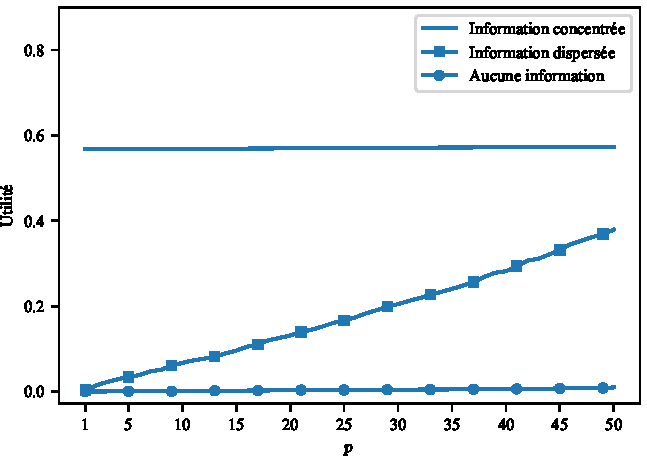
\includegraphics[width=\textwidth]{../../experiments/fig/pconst_euinforelative.pdf}
  \caption{Progression de $EU^\star$ relatif}
  \label{fig_pconst_euinforelative}
\end{figure}

\begin{figure}[h!]
  \centering
  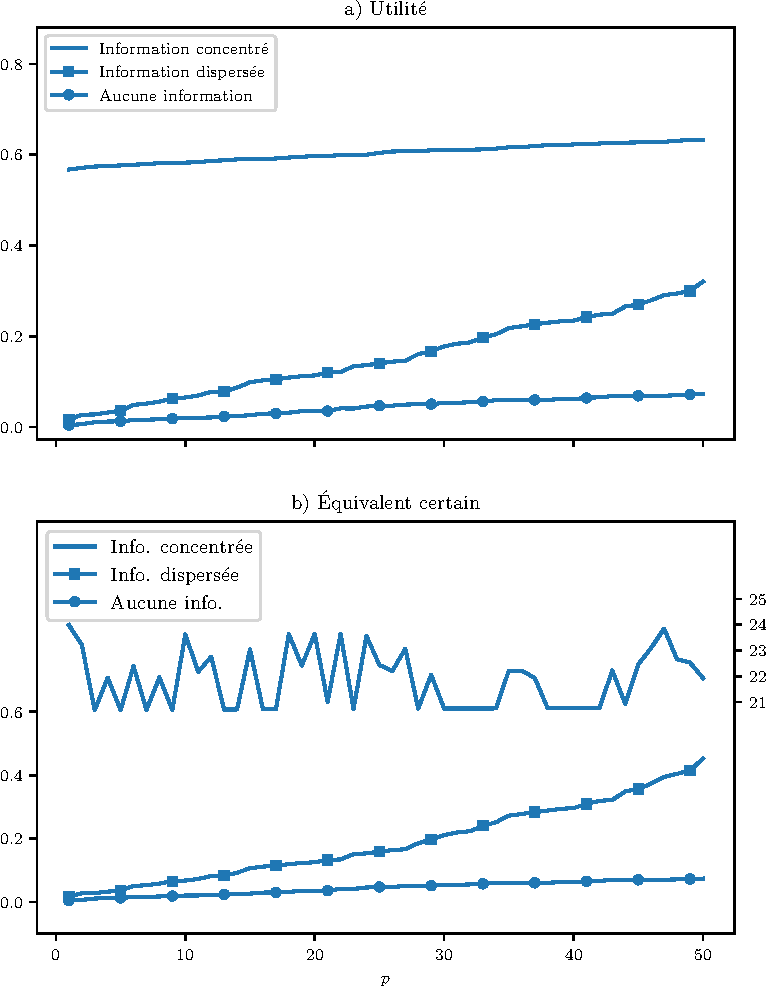
\includegraphics[width=\textwidth]{../../experiments/fig/pconst_infosorelative.pdf}
  \caption{Progression de la sous optimalité relative}
  \label{fig_pconst_infosorelative}
\end{figure}

\begin{figure}[h]
  \centering
  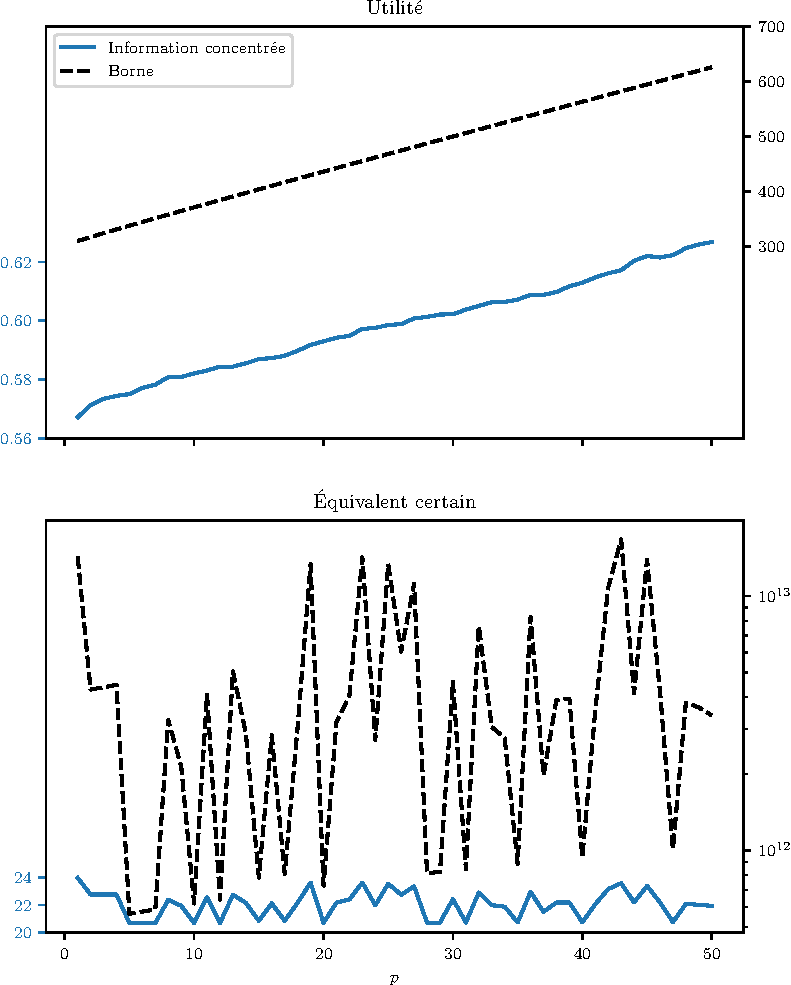
\includegraphics[width=\textwidth]{../../experiments/fig/pconst_so_conc.pdf}
  \caption[Borne sur l'erreur de S.O. I]{Borne sur l'erreur de sous optimalité,
    information concentrée}
  \label{fig_pconst_so_conc}
\end{figure}

\begin{figure}[h]
  \centering
  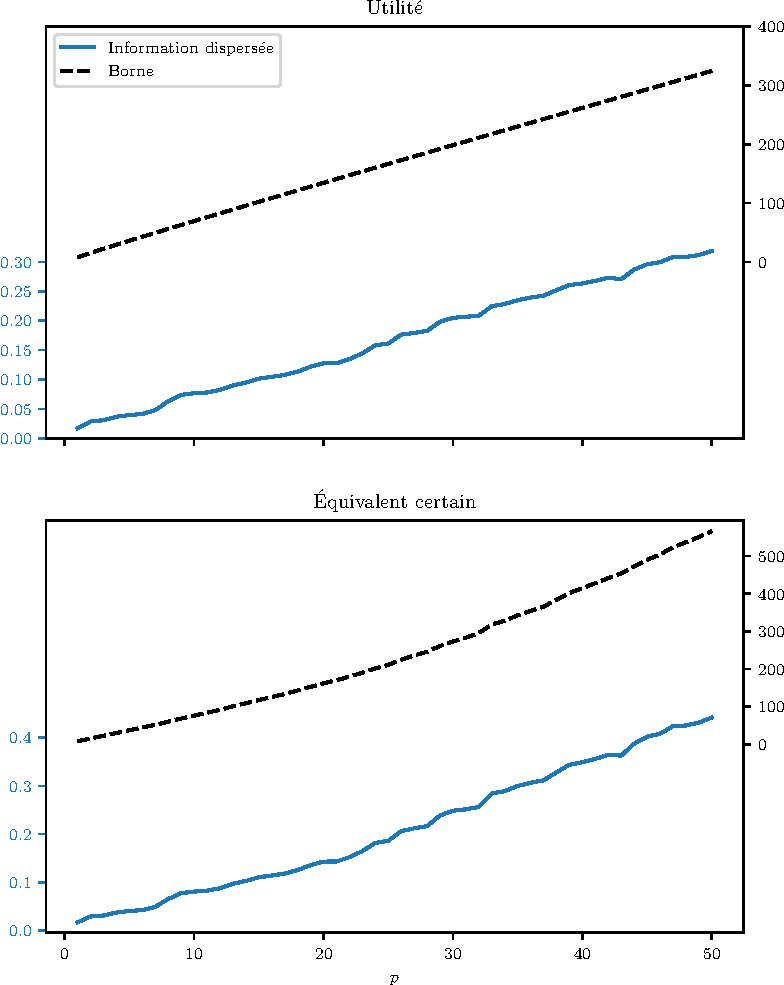
\includegraphics[width=\textwidth]{../../experiments/fig/pconst_so_disp.pdf}
  \caption[Borne sur l'erreur de S.O. II]{Borne sur l'erreur de sous optimalité,
    information dispersée}
  \label{fig_pconst_so_disp}
\end{figure}

\begin{figure}[h]
  \centering
  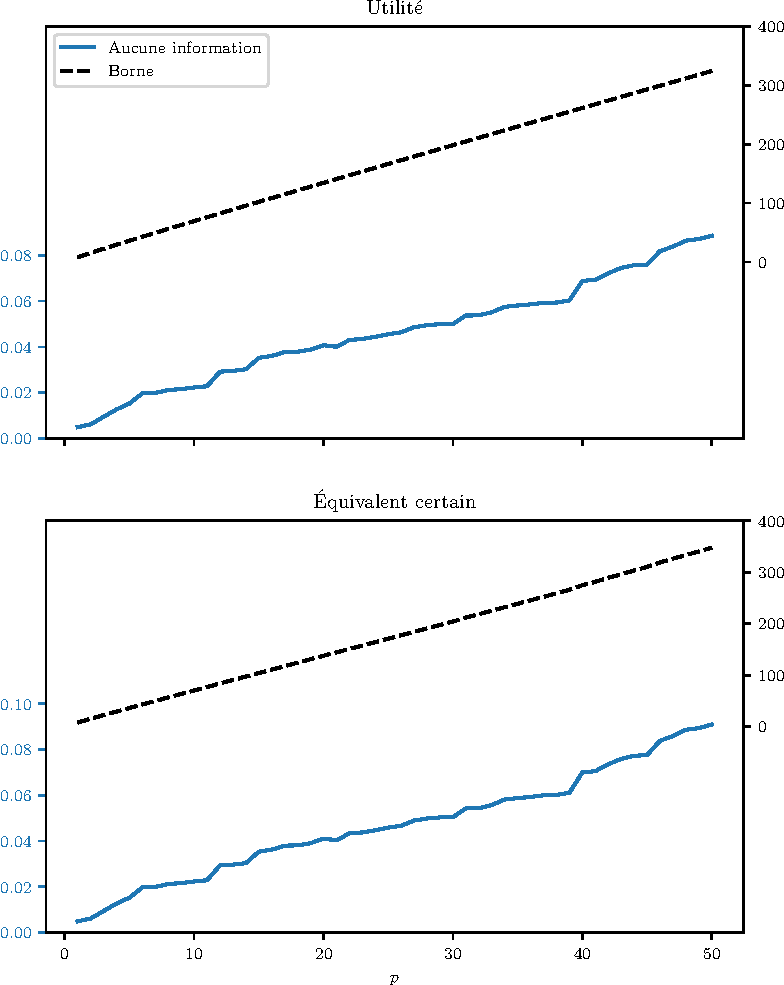
\includegraphics[width=\textwidth]{../../experiments/fig/pconst_so_auc.pdf}
  \caption[Borne sur l'erreur de S.O. III]{Borne sur l'erreur de sous optimalité, aucune
    information}
  \label{fig_pconst_so_auc}
\end{figure}

\clearpage

\subsection{Ajout d'information et d'échantillons}
\label{emp:npvar}

Cette section cherche à illustrer les comportements des deux bornes lorsqu'on est en
présence de régimes dynamiques en $n$ et en $p$, \ie\ lorsque $p=\O(n^k)$.

\paragraph{Méthodologie}

Cette fois, la loi de marché théorique $\tilde M$ disposera de $\bar p=100$ variables
d'information, encore liées à $R$ à partir d'une copule gaussienne $\Sigma$ donnée par
\begin{equation}
  \Sigma =
  \kbordermatrix{
    &X_1 & \cdots & X_{\bar p} & R\\
    X_1& \ddots & & & \rotatebox{90}{\text{---}}\\
    \vdots  & & I_{\bar p\times \bar p} && \rho\\
    X_{\bar p}&&&\ddots &\rotatebox{90}{\text{---}}\\
    R & \text{---} & \rho & \text{---} &1}.
\end{equation}
où cette fois,
$\rho = \left(\begin{smallmatrix}1/\sqrt{100} & \cdots &1/\sqrt{100}\end{smallmatrix}\right)$.

Trois régimes seront étudiés : celui où $p=\bigO(n^{1/2})$, $p=\bigO(n^{3/4})$ et
$p=\bigO(n)$. À des fins de simplicité, chacun de ces régimes sera décrit par la puissance
$k$ de $n$, de manière à avoir $k=1/2,3/4$ et $1$. La figure \ref{fig_np_np} illustre
précisément les trois régimes.

\begin{figure}[h]
  \centering
  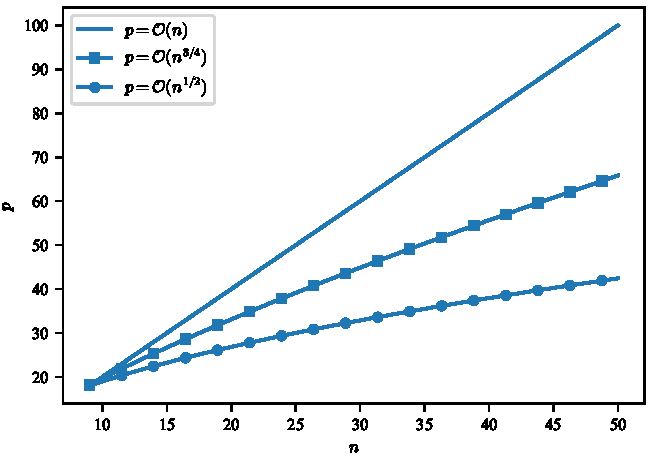
\includegraphics[width=0.7\textwidth]{../../experiments/fig/np_np.pdf}
  \caption{Progression de $p$ par rapport à $n$}
  \label{fig_np_np}
\end{figure}

\subsubsection{Erreur de généralisation}

\paragraph{Borne de généralisation -- Figure \ref{fig_np_genbound}}

La \figref{fig_np_genbound} illustre enfin le problème avec la théorie présentée jusqu'à
présent. Jusqu'à présent, même si les bornes théoriques dérivées n'étaient pas
nécessairement serrées, elles servaient tout de même de guide pour connaître le régime
dans lequel l'erreur empirique progressait. Par exemple, lorsque $p$ était fixe, on
obtenait systématiquement une erreur de généralisation décroissant avec un rythme
$\bigO(n^{-1/2})$. De la même façon, avec $n$ constant, ces mêmes erreurs évoluaient selon
un régime $\bigO(p)$. On se serait donc attendu à ce qu'on obtienne un régime global
d'erreur $\bigO(p/\sqrt{n})$. Cependant, la \figref{fig_np_genbound} démontre clairement
que tel n'est pas le cas, puisque peu importe le régime, là où on se serait attendu soit
au moins à une erreur constante, on observe plutôt une diminution de l'erreur de
généralisation!

\paragraph{Régime d'ordre plus élevé -- Figure \ref{fig_np_gen32}}

Il faut effectivement attendre de voir apparaître des régimes très élevés (par exemple
$k=3/2$) avant d'enfin observer une augmentation de l'erreur. Cependant, l'ordre exact $k$
ne semble pas clair et certaines expériences laissent croire que $k$ pourrait plutôt
dépendre des paramètres du problème.


\subsubsection{Erreur de sous optimalité}

La Figure \ref{fig_np_sobound} présente quant à elle l'erreur de sous optimalité pour les
trois régimes étudiés et une fois encore, on constate une vive différence entre l'ordre
donné par la borne théorique et ce qu'on observe en pratique. La courbe empirique $k=1/2$
à peu près stable laisse croire qu'on est en présence d'un régime $\bigO(p/\sqrt{n})$,
mais la courbe $k=1$ vient en fait démentir cette interprétation puisque la progression
paraît alors linéaire, un peu comme ce qui était observé lorsque $n$ était constant.

De plus, la forme même des bornes théoriques permet de constater les deux régimes
théoriques superposés, c'est-à-dire de la forme $\bigO(p/n + p/\sqrt{n})$. Par ailleurs,
la présence du terme de régularisation vient une fois de plus brouiller les
interprétations, puisqu'il faut conserver à l'esprit qu'un terme $\lambda\|q^\star\|^2$ est aussi compris
dans la borne, et dont la progression est encore mal comprise (voir \figref{fig_np_normqp}).


\begin{figure}[h]
  \centering
  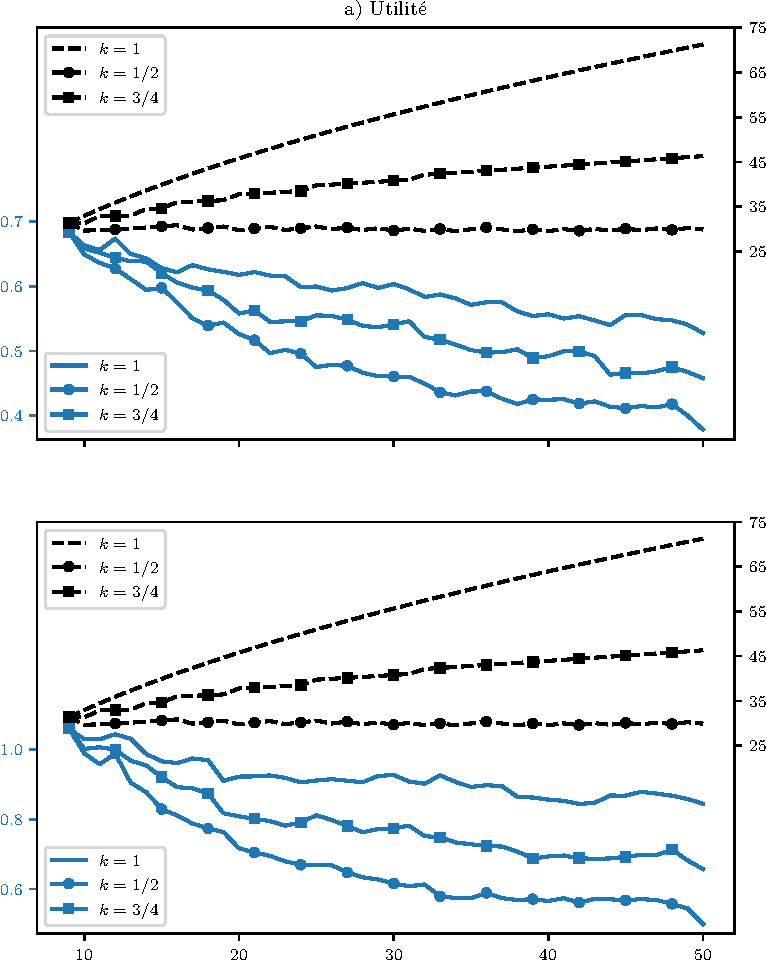
\includegraphics[width=\textwidth]{../../experiments/fig/np_genbound.pdf}
  \caption[à faire]{Borne sur l'erreur de généralisation, $n$ et $p$ variables}
  \label{fig_np_genbound}
\end{figure}

\begin{figure}[h]
  \centering
  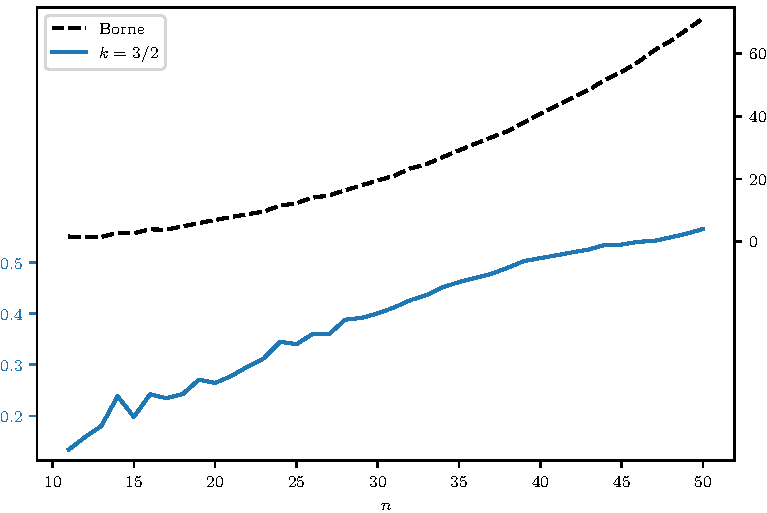
\includegraphics[width=\textwidth]{../../experiments/fig/np_gen32.pdf}
  \caption{Erreur de généralisation à très haut régime}
  \label{fig_np_gen32}
\end{figure}

\begin{figure}[h]
  \centering
  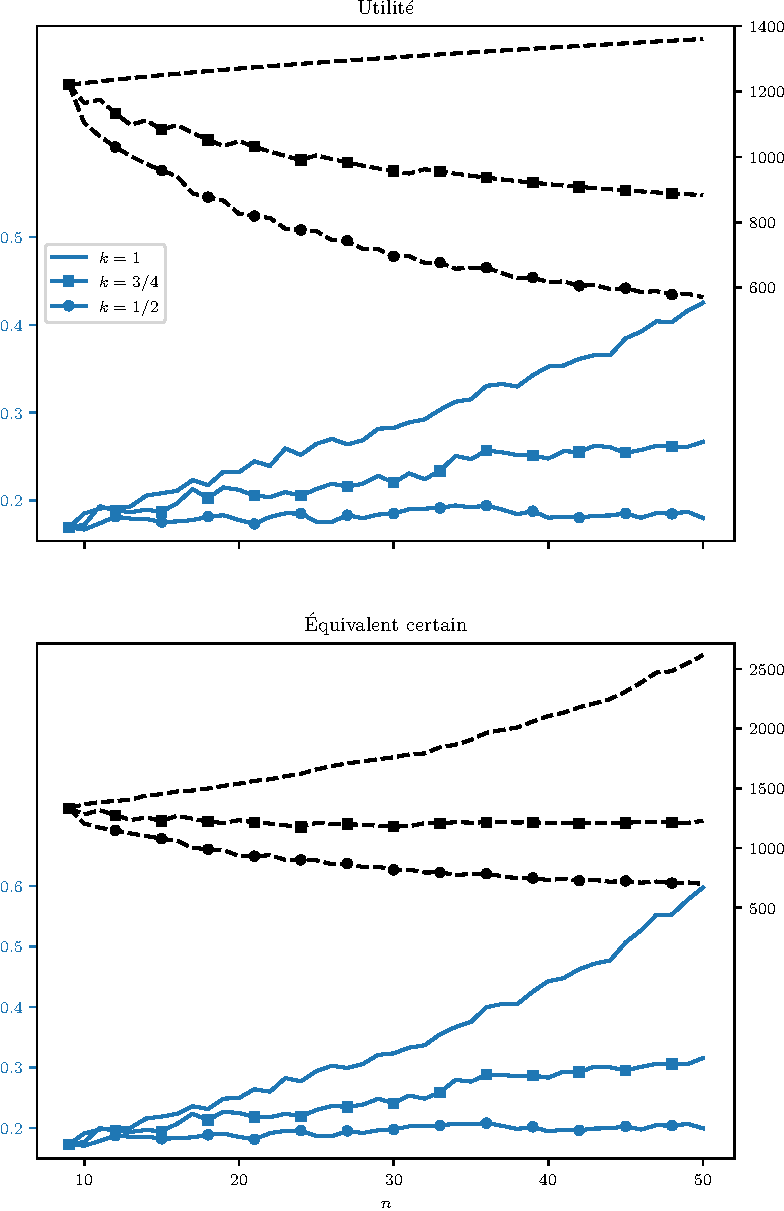
\includegraphics[width=\textwidth]{../../experiments/fig/np_sobound.pdf}  
  \caption[à faire]{Borne sur l'erreur de sous-optimalité, $n$ et $p$ variables}
  \label{fig_np_sobound}
\end{figure}

\begin{figure}[h]
  \centering
  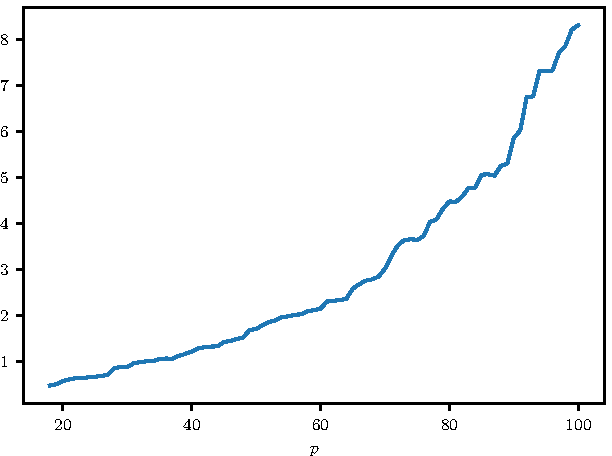
\includegraphics[width=\textwidth]{../../experiments/fig/np_normqp.pdf}
  \caption{Progression de $\|q^\star\|^2$}
  \label{fig_np_normqp}
\end{figure}

\clearpage

% \begin{table}[h]
%   \small
%   \centering
% \begin{tabular}{lrrr}
% \toprule
% $n$ &   $k=1/2$ &  $k=3/4$ &   $k=1$ \\
% \midrule
% 2  &   3 &   4 &   5 \\
% 3  &   4 &   5 &   7 \\
% 4  &   5 &   7 &  10 \\
% 5  &   5 &   8 &  12 \\
% 6  &   6 &   9 &  15 \\
% 7  &   6 &  10 &  17 \\
% 8  &   7 &  11 &  20 \\
% 9  &   7 &  12 &  22 \\
% 10 &   7 &  14 &  25 \\
% 11 &   8 &  15 &  27 \\
% 12 &   8 &  16 &  30 \\
% 13 &   9 &  17 &  32 \\
% 14 &   9 &  18 &  35 \\
% 15 &   9 &  19 &  37 \\
% 16 &  10 &  20 &  40 \\
% 17 &  10 &  20 &  42 \\
% 18 &  10 &  21 &  45 \\
% 19 &  10 &  22 &  47 \\
% 20 &  11 &  23 &  50 \\
% 21 &  11 &  24 &  52 \\
% 22 &  11 &  25 &  55 \\
% 23 &  11 &  26 &  57 \\
% 24 &  12 &  27 &  60 \\
% 25 &  12 &  27 &  62 \\
% 26 &  12 &  28 &  65 \\
% 27 &  12 &  29 &  67 \\
% 28 &  13 &  30 &  70 \\
% 29 &  13 &  31 &  72 \\
% 30 &  13 &  32 &  75 \\
% 31 &  13 &  32 &  77 \\
%   \bottomrule
% \end{tabular}
% \caption{Progression de $p$ par rapport à $n$}
% \label{tbl_np_np}
% \end{table}


% \begin{figure}
%   \centering
%   \caption{Progression de $p$ par rapport à $n$}
%   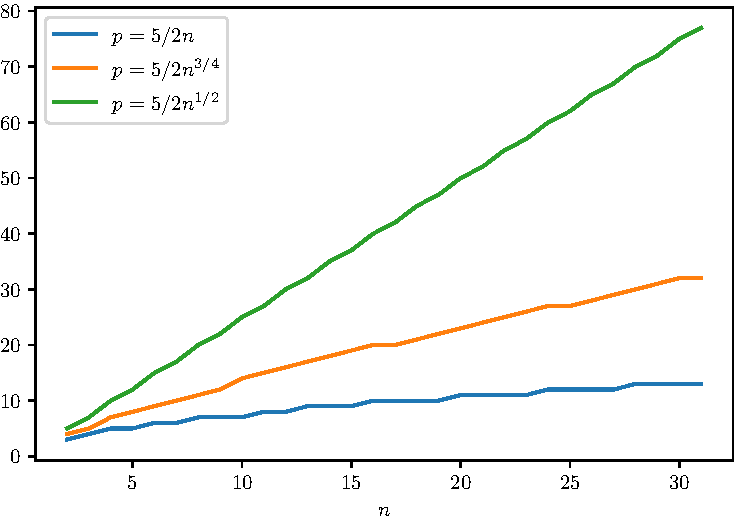
\includegraphics[width=0.8\textwidth]{../../experiments/fig/progression1.pdf}
% \end{figure}


% \begin{figure}
%   \centering
%   \begin{subfigure}[b]{\textwidth}
%     \centering
%     \caption{Domaine de l'utilité}
%     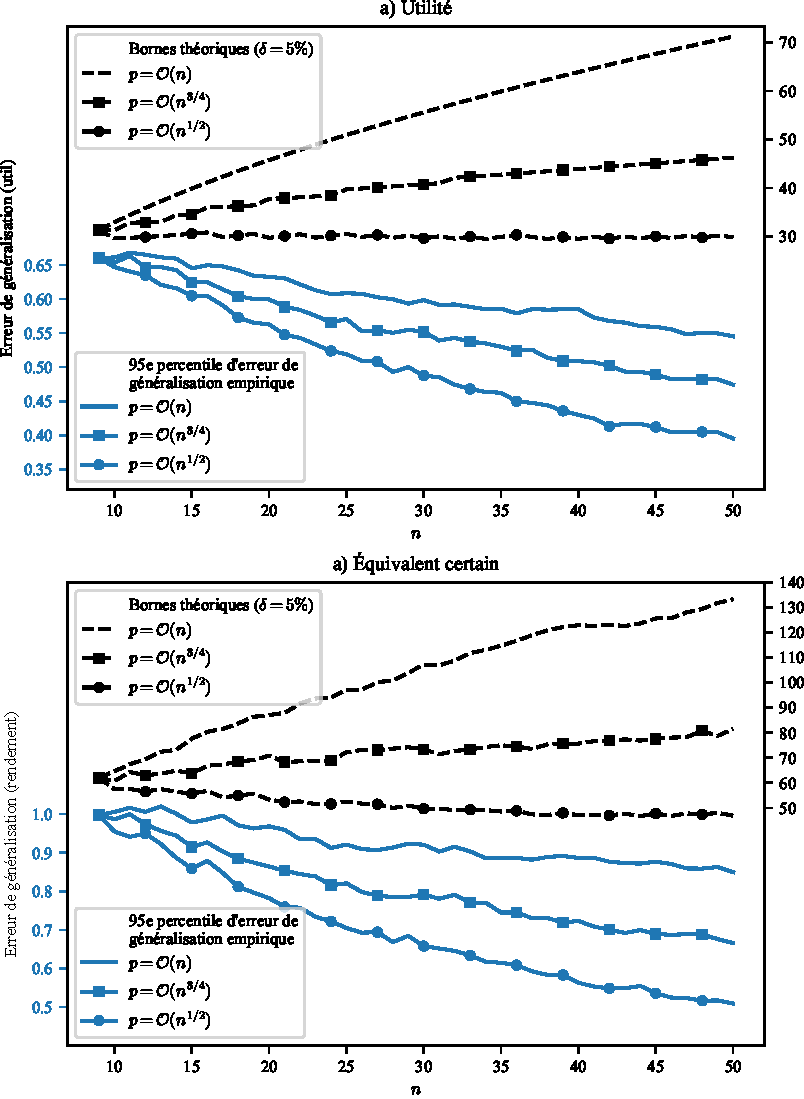
\includegraphics[width=\textwidth]{../../experiments/fig/bound_npgenu.pdf}
%   \end{subfigure}
%   \hfill
%   \begin{subfigure}[b]{0.8\textwidth}
%     \caption{Domaine des rendements}
%     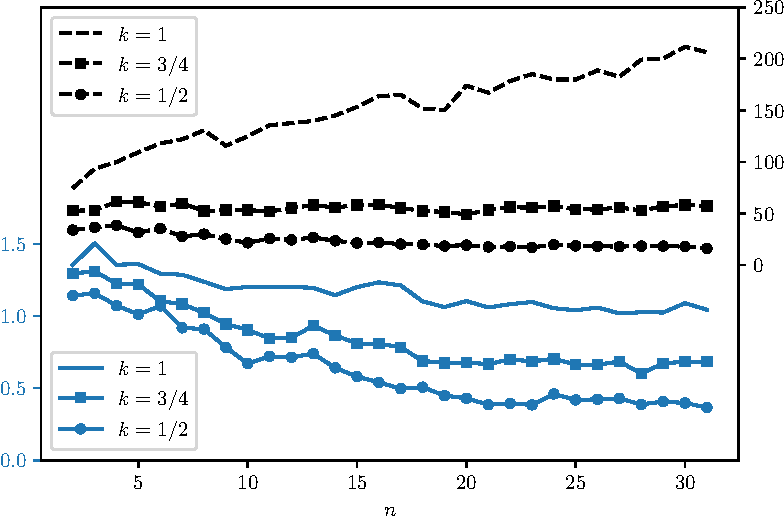
\includegraphics[width=\textwidth]{../../experiments/fig/bound_npgence.pdf}
%   \end{subfigure}
%   \caption{Erreur de généralisation -- $n$ et $p$ variables}
%   \label{fig_bound_genu}
% \end{figure}



%%% Local Variables:
%%% mode: latex
%%% TeX-master: "../memoire/memoire"
%%% End:
